%!TEX root = PMP_ClockPendulumAnalyzer.tex
\section{Projektrahmenplan}
    In diesem Kapitel werden die Meilensteine und Eckdaten wie Start- und Endzeitpunkt des Projekts festgehalten.
    \begin{figure}[H]
        \centering
        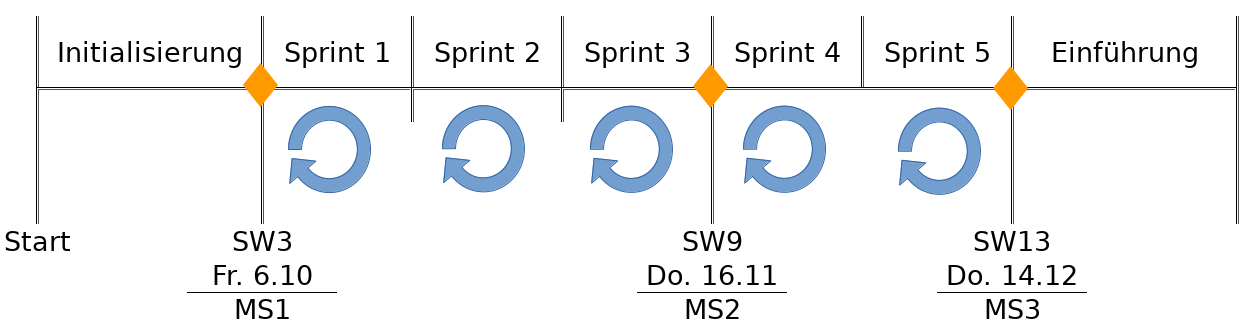
\includegraphics[width=\textwidth]{rahmenplan.png}
        \caption{Rahmenplan mit Phasen, Meilensteine und Sprints}
    \end{figure}
    \begin{tabularx}{\textwidth}{lll}
        \textbf{MS1} & Zeitpunkt: & Freitag 6.10.\\
        & Artefakte: & \tabitem PMP\\
        & & \tabitem Entwurf des Grobkonzepts\\
        & Ergebnisse: & \tabitem definierte Vorgehensart\\
        & & \tabitem Rahmenplanung\\
        & & \tabitem Vision (Scope, Ziele etc) im Grobkonzept\\
        \textbf{MS2} & Zeitpunkt: & Donnerstag 16.11.2017\\
        & Artefakte & \tabitem Prototyp 1\\
        & Ergebnisse: & \tabitem lauffähiger 1. Prototyp\\
        & & \tabitem 80\% der Sys Spec\\
        \textbf{MS3} & Zeitpunkt: & Donnerstag 14.12.2017\\
        & Artefakte & \tabitem PMP \\
        & & \tabitem SysSpec \\
        & & \tabitem Arbeitsjournal \\
        & & \tabitem Prototyp 2\\
        & Ergebnisse: & \tabitem lauffähiger 2. Prototyp\\
        & & \tabitem fertige System Spezifikation (Projektreport)\\
        & & \tabitem fertiger PMP\\
    \end{tabularx}